% This material is copyright Simon Dobnik and made available under the
% Creative Commons Attribution 4.0 International License (CC-BY-SA)
% license http://creativecommons.org/licenses/by-sa/4.0/
% 
% Email: simon.dobnik@gu.se
% Web: http://dobnik.net/simon/teaching/shared/LT2112-formling/


\documentclass{beamer}

\usepackage{graphicx,color,hyperref,avm,fullname,qtree}
\usepackage[utf8]{inputenc} 




\logo{
\includegraphics[height=0.5cm]{pics/GU-logo.pdf}} 
\newcommand{\bblue}[1]{{\usebeamercolor[fg]{frametitle}{#1}}}


\definecolor{links}{HTML}{2A1B81}
\hypersetup{colorlinks,linkcolor=,urlcolor=links}

\setbeamertemplate{footline}[frame number]



\AtBeginSection[]
{
\begin{frame}[plain]

{\huge\bblue{\insertsectionhead}}

\end{frame}
}




\setlength\fboxrule{1pt}
\setlength\fboxsep{0mm} 





\title{Introduction to Formal Linguistics}

\author{Simon Dobnik\\
Department of Philosophy, Linguistics and Theory of Science}

\date{September 3, 2015}





\begin{document}

\frame[plain]{\titlepage

\centering{Based on slides by Robin Cooper}

}





\frame[plain]{\frametitle{Outline}\tableofcontents}





\section{Practicalities}

\frame{

\frametitle{The course website}

LT2112 H15 Introduction to formal linguistics on \href{https://gul.gu.se}{https://gul.gu.se}

\bigskip

\href{https://gul.gu.se/courseId/70822/content.do?id=30160898}{https://gul.gu.se/courseId/65958/content.do?id=26978419}

\bigskip

\href{http://gul.gu.se/public/courseId/70822/lang-en/publicPage.do}{http://gul.gu.se/public/courseId/70822/lang-en/publicPage.do}

\bigskip


\includegraphics[scale=0.1]{pics/course-webpage.png}

}





\frame{

\frametitle{Course lecturers}

\begin{itemize} 

\item \href{http://flov.gu.se/om/personal/ellen-breitholtz}{Ellen Breitholtz} \\(morphology)
 
\item \href{http://www.flov.gu.se/english/contact/staff/dobnik-simon/}{Simon Dobnik} \\(syntax and semantics with pragmatics, course organiser)

\item \href{http://flov.gu.se/om/personal/johan-gross}{Johan Gross} \\(phonetics and phonology)
 
\end{itemize} 
  
}





\section{Overview of linguistics}

\frame{

\frametitle{Linguistics -- a scientific view of language}

\begin{itemize} 
 
\item formal: explicit, exact (to an extent) 
 
\pause \item \href{http://en.wikipedia.org/wiki/Noam_Chomsky}{Noam Chomsky}, starting mid-fifties  

\pause \item but goes back to ancient grammarians (\href{http://en.wikipedia.org/wiki/P\%C4\%81\%E1\%B9\%87ini}{P\={a}\d{n}ini}, 4th
  cent. B.C.)

\pause \item nineteenth century (historical perspective, diachronic, \href{http://en.wikipedia.org/wiki/Hermann_Paul}{Hermann Paul:} sentences are the sum of their parts)

\pause \item pre-Chomskyan 20th century -- synchronic (\href{http://en.wikipedia.org/wiki/Ferdinand_de_Saussure}{Saussure}),
  structuralists (\href{http://en.wikipedia.org/wiki/Leonard_Bloomfield}{Leonard Bloomfield}, \href{http://en.wikipedia.org/wiki/Charles_Hockett}{Charles Hockett}, \href{http://en.wikipedia.org/wiki/Zellig_Harris}{Zellig Harris})











 

\end{itemize} 
}





\frame{

\frametitle{Linguistic methods}

\bigskip

\begin{itemize} 
 
\item corpus linguistics 
 
\item formal analysis

\item experimental methods
 
\end{itemize} 
  

}





\begin{frame}

\frametitle{Computational linguistics}

\ldots the scientific study of human language -- specifically of the system of rules and the ways in which they are used in communication -- using mathematical models and formal procedures that can be realised and validated using computers; a cross-over of many disciplines. (Stanford Linguistics Professor, 1980s) 

\hfill \footnotesize Borrowed from Stephan Oepen's slide

\end{frame}





\begin{frame}

\frametitle{Computational Linguistics}


\href{https://en.wikipedia.org/wiki/Computational_linguistics}{Wikipedia}

\bigskip

\href{http://www.coli.uni-saarland.de/~hansu/what_is_cl.html}{University of Saarland}


\end{frame}





\frame{

\frametitle{A language module}

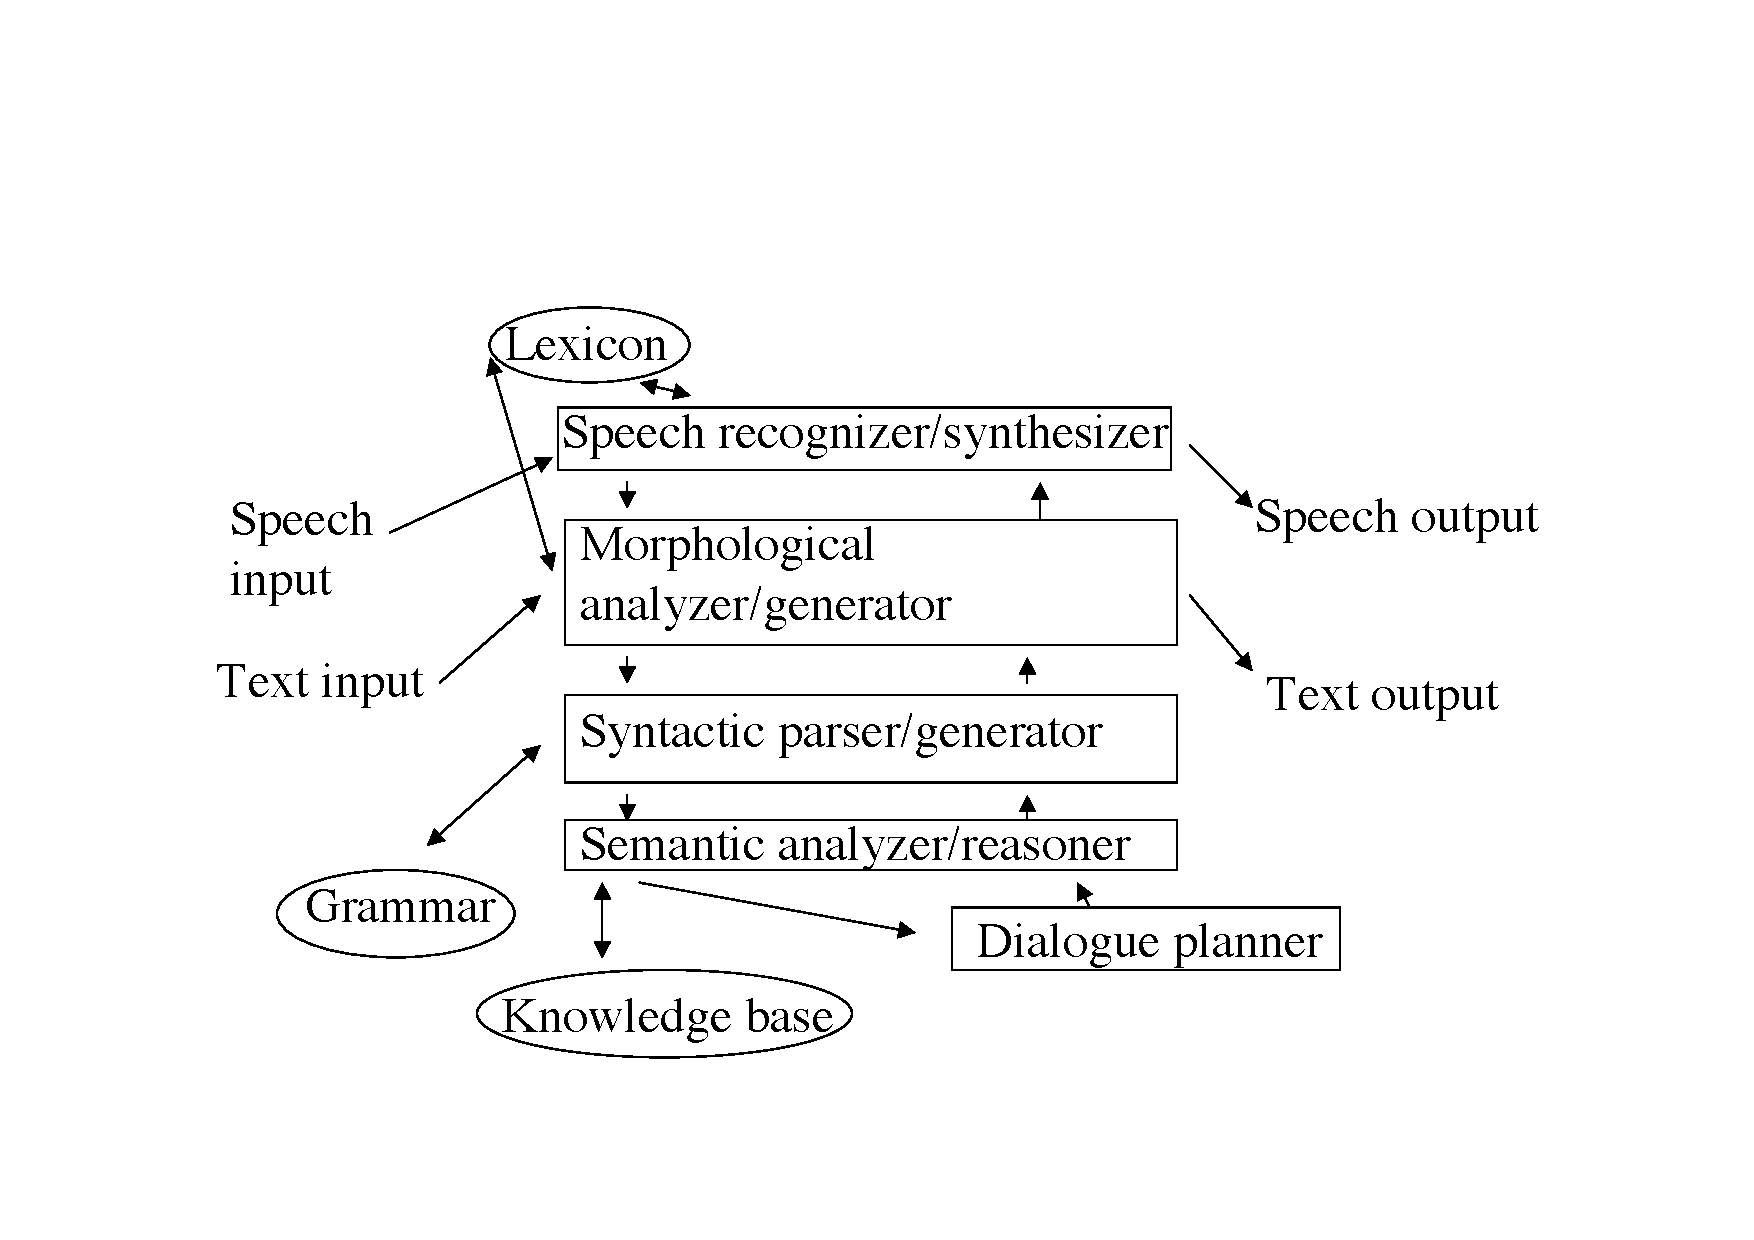
\includegraphics[width=\textwidth]{pics/langmodule}


}





\section{Phonetics and Phonology}

\frame{

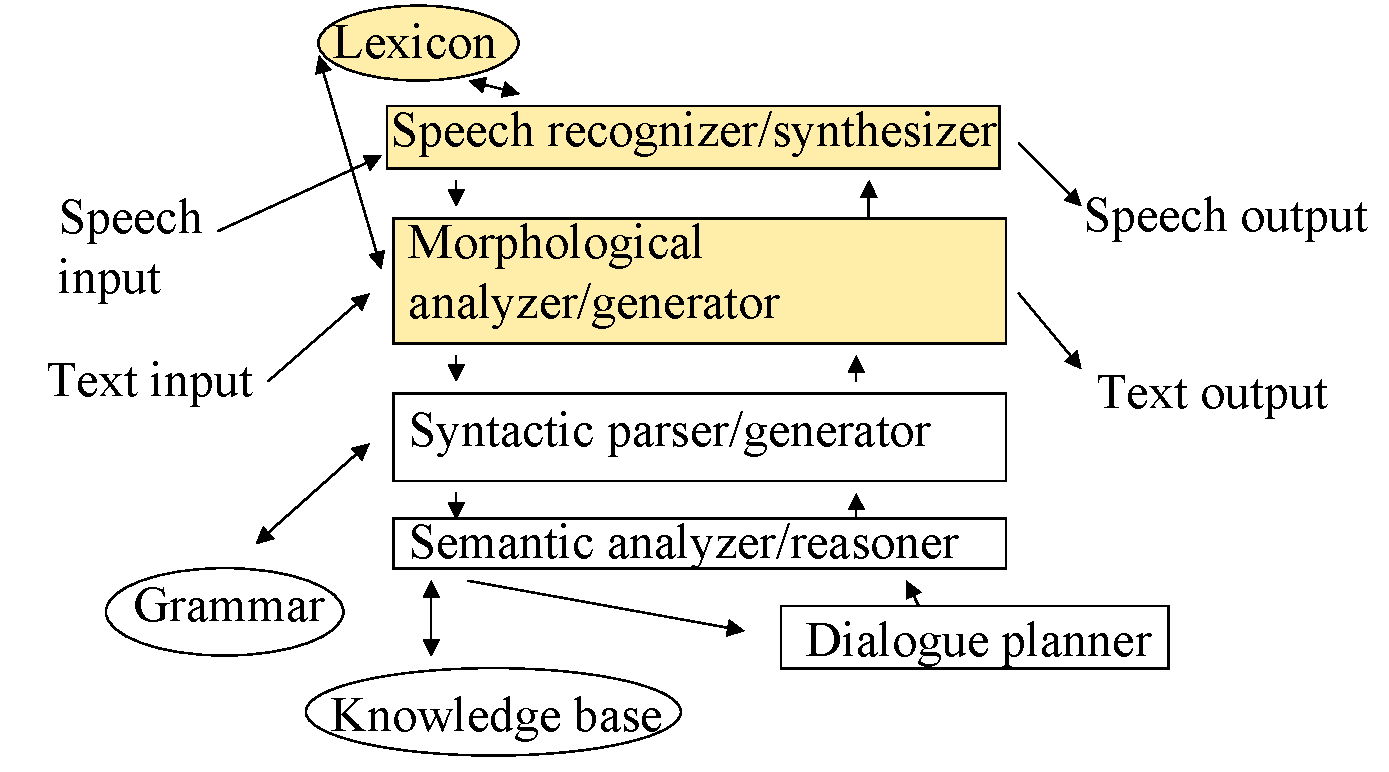
\includegraphics[width=\textwidth]{pics/phonphon}

}





\frame{

\frametitle{Articulatory phonetics}

\begin{itemize} 
 
\item how we use our mouth, vocal tract to produce speech sounds 
 
\pause \item classification of speech sounds according to articulation 
 
\end{itemize} 
  

}





\frame{

\frametitle{The vocal tract}

\begin{center}
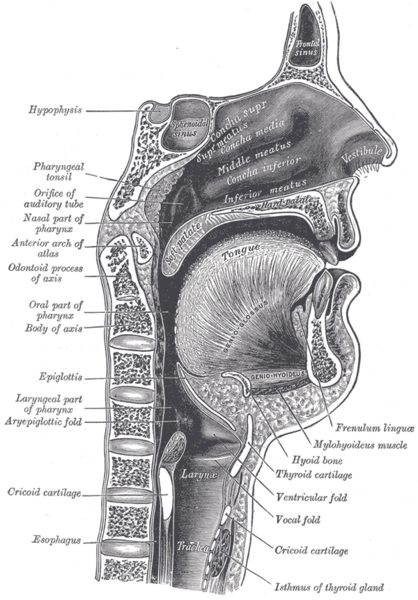
\includegraphics[scale=0.33]{pics/vocal-tract}

From \href{http://en.wikipedia.org/wiki/Vocal_tract}{Wikipedia}.
\end{center}


}





\frame{

\frametitle{The IPA chart}

\href{http://www.internationalphoneticalphabet.org/ipa/}{http://www.internationalphoneticalphabet.org/ipa/}

\begin{center}
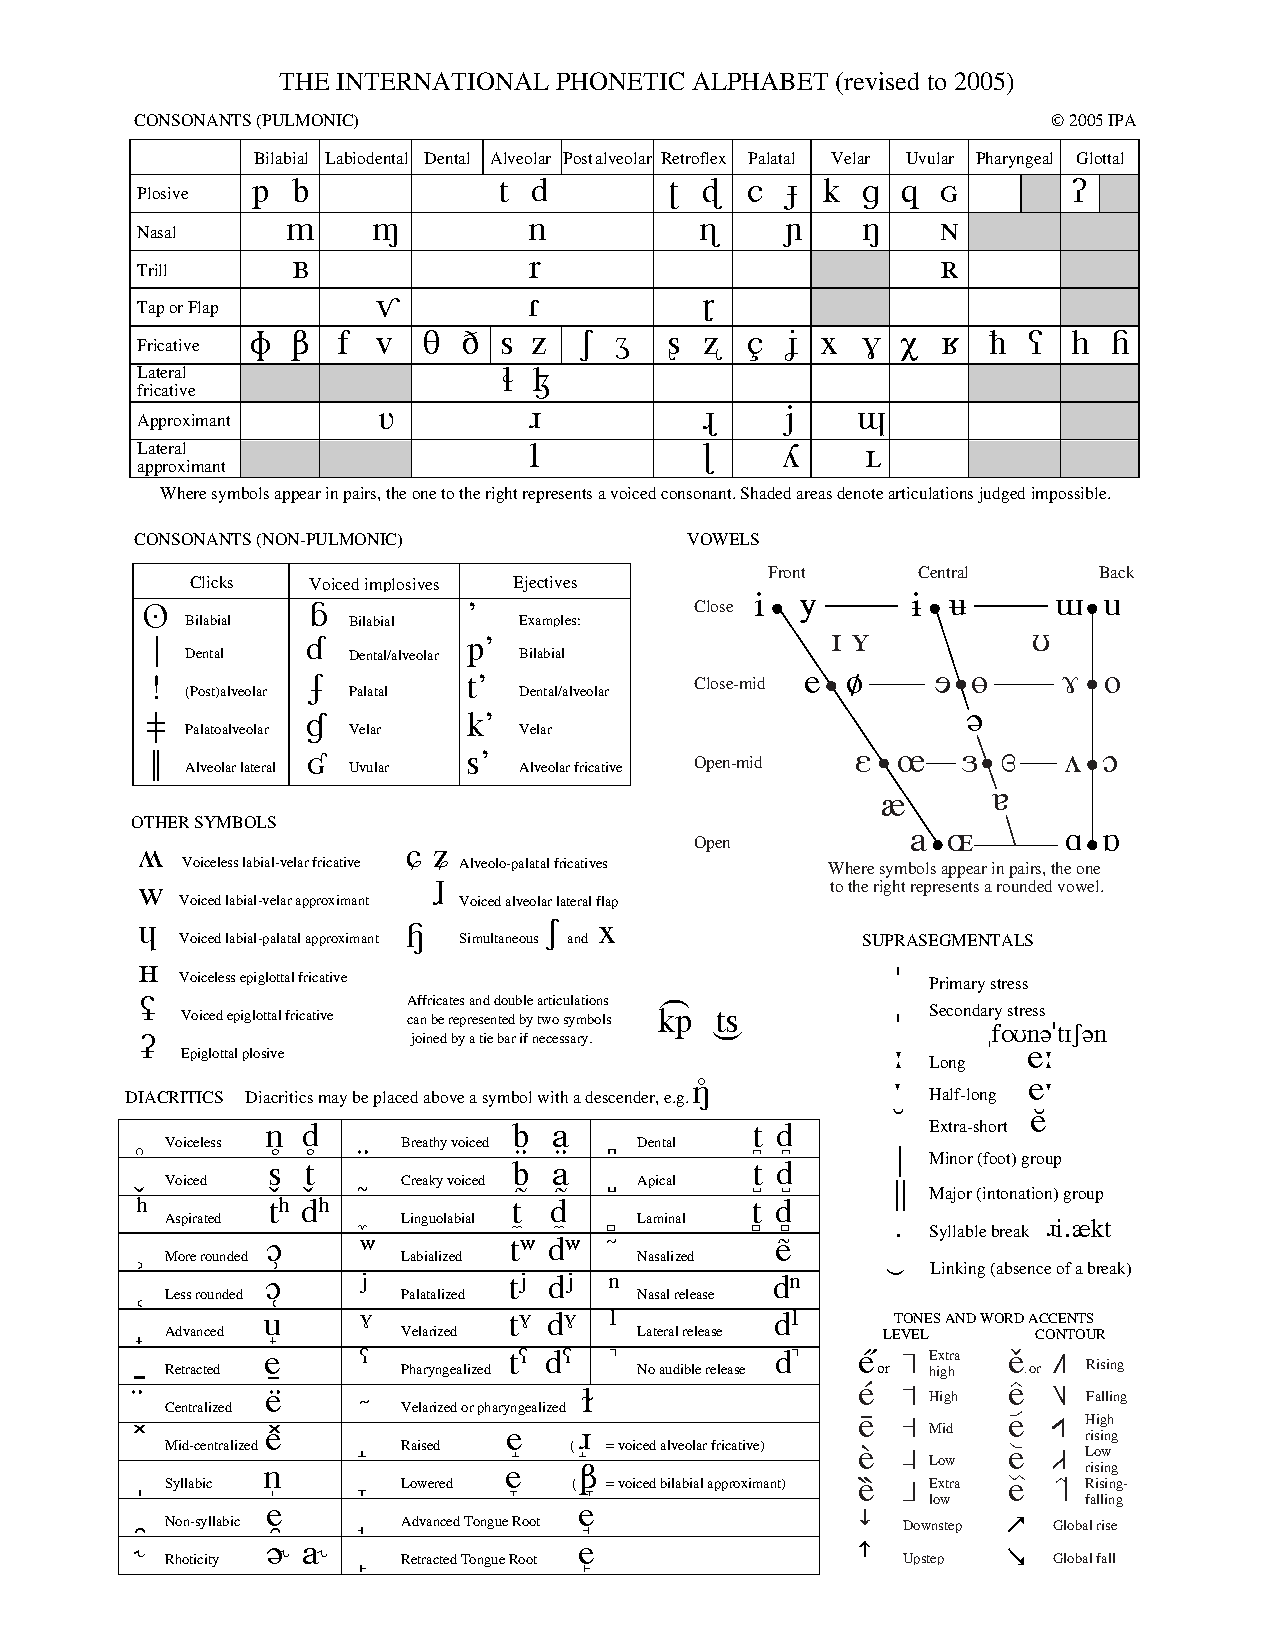
\includegraphics[scale=0.25]{pics/IPA_chart_(C)2005.pdf}
\end{center}

}





\frame{

\frametitle{The IPA chart for pulmonic consonants}


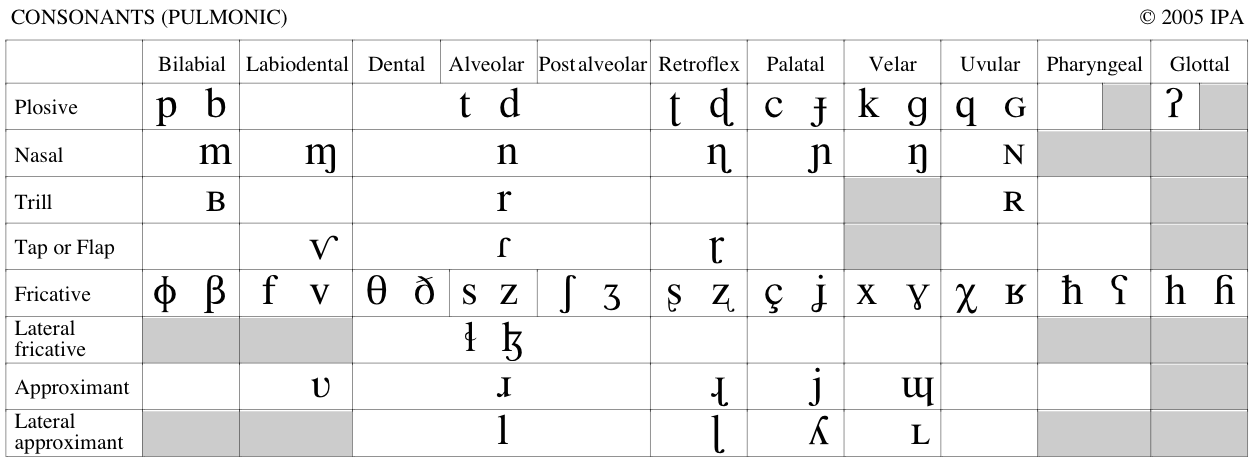
\includegraphics[width=\textwidth]{pics/ipa-pulmonic-consonants.png}

}





\begin{frame}

\frametitle{The IPA chart for vowels}

\begin{center}
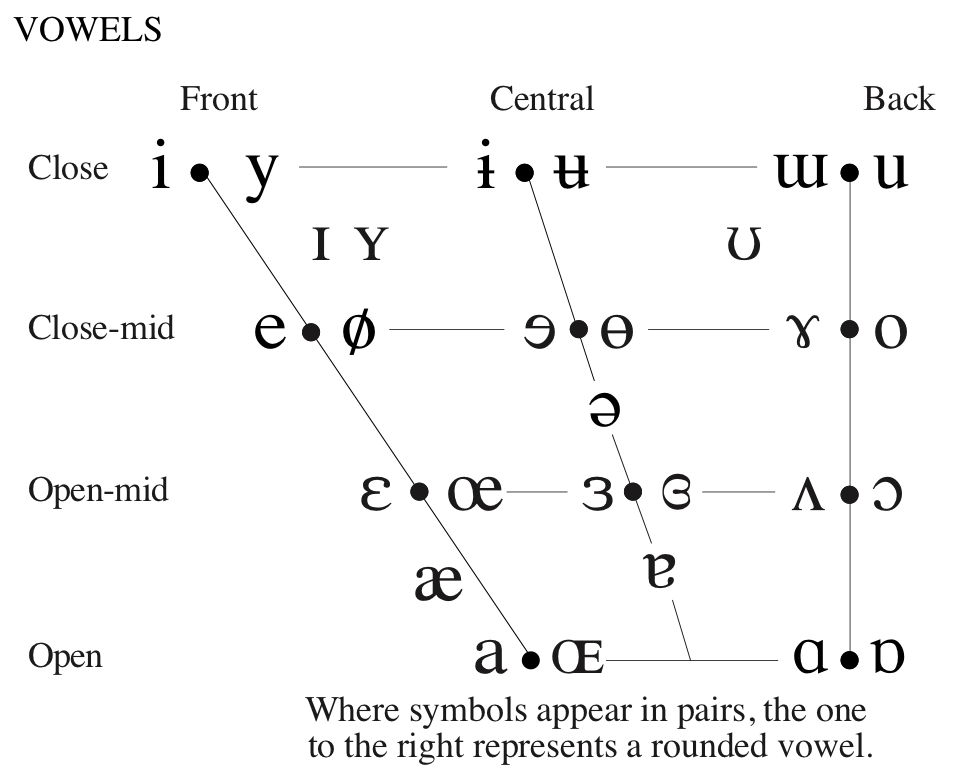
\includegraphics[width=0.65\textwidth]{pics/ipa-vowels.png}
\end{center}

\end{frame}





\frame{

\frametitle{Acoustic phonetics}

\begin{itemize} 
 
\item the data from sound waves 
 
\pause \item can we recognise speech sounds from the acoustic data?

\pause \item not just acoustic data: \href{http://en.wikipedia.org/wiki/McGurk_effect}{McGurk effect}, \href{http://www.youtube.com/watch?v=G-lN8vWm3m0}{video}

\pause \item continuous speech to discrete speech sounds, co-articulation
 
\end{itemize} 
  

}





\frame{

\frametitle{Spectrogram}

\begin{center}
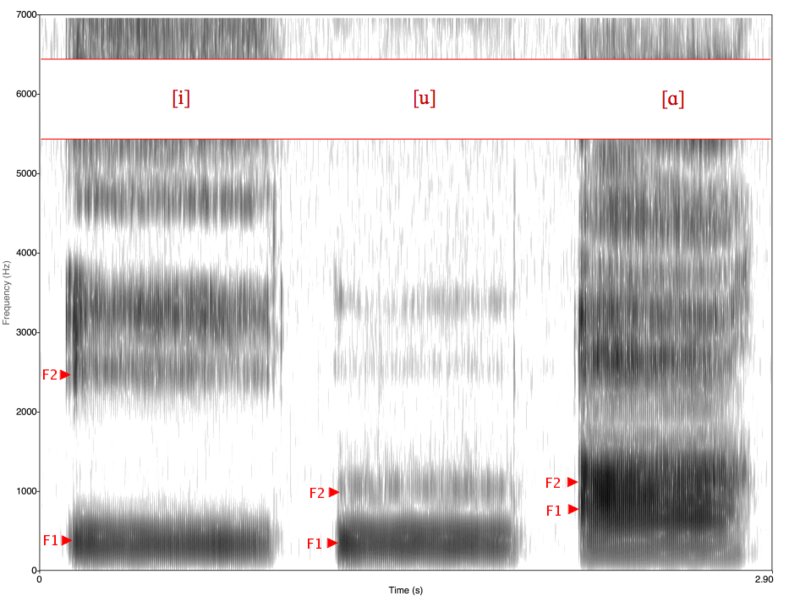
\includegraphics[scale=1.5]{pics/spectrogram}

From \href{http://en.wikipedia.org/wiki/Formant}{Wikipedia}.
\end{center}

}





\frame{

\frametitle{Phonology}

\begin{itemize} 
 
\item phonemes (\textit{kit}, \textit{cat}) 
 
\pause \item phonological rules (\textit{[s]ip},\textit{[z]ip} \pause --
  \textit{sip[s]}, \textit{zip[s]} $\approx$ \textit{bib[z]}, \textit{pub[z]})
 
\end{itemize} 


}





\section{Morphology}


\frame{

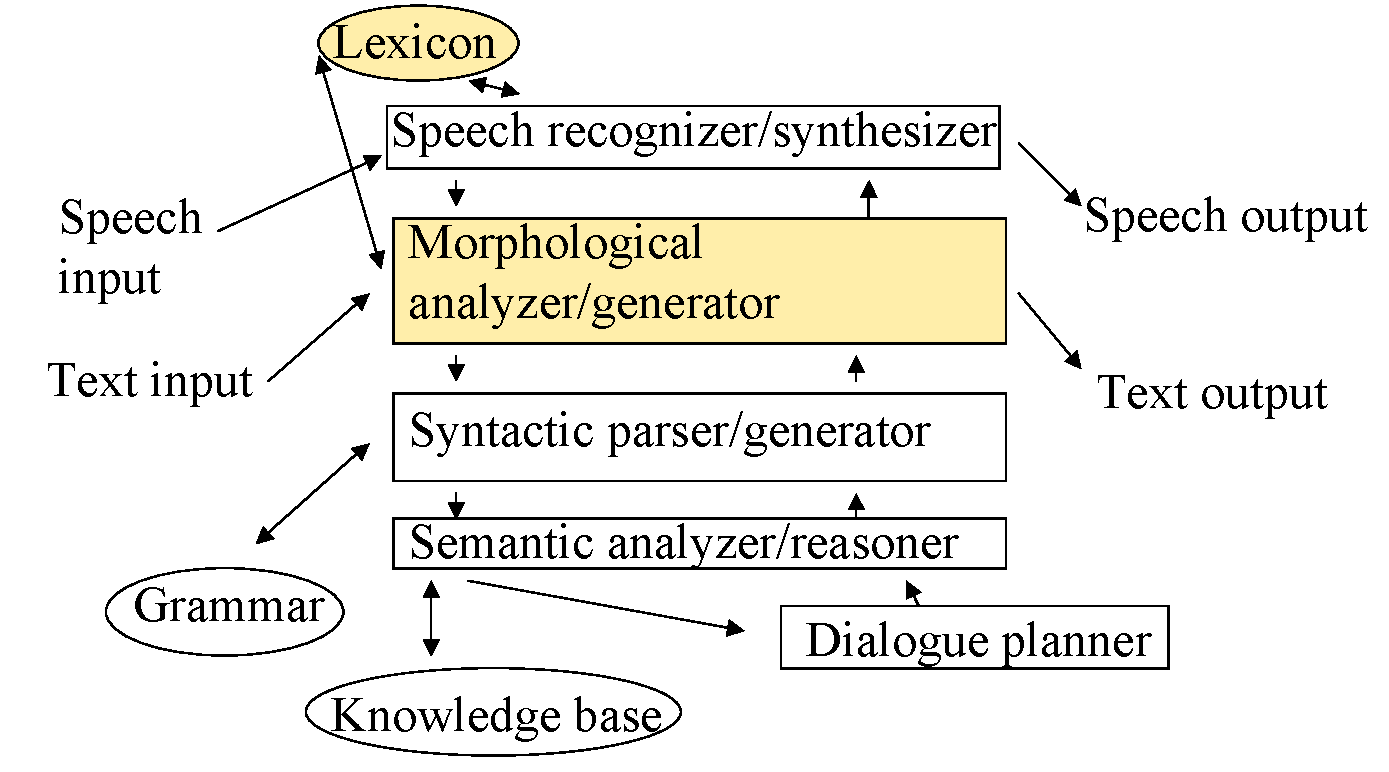
\includegraphics[width=\textwidth]{pics/morph}

}

\frame{

\frametitle{Inflectional morphology}

\begin{itemize} 
 
\item different forms in a paradigm 
 
\item singular vs plural (\textit{cat} vs \textit{cats}, \textit{run},
  \textit{runs}, \textit{ran}) 
 
\end{itemize} 
  

}





\frame{

\frametitle{Derivational morphology}

\begin{itemize} 
 
\item creating new words, perhaps of a different category, perhaps
  with a different meaning 
 
\item \textit{clever} $\approx$ \textit{cleverness}, \textit{able}
  $\approx$ \textit{ability} 
 
\end{itemize} 
  

}





\frame{

\frametitle{Other morphological processes}

\begin{itemize} 
 
\item not clear if there is a clear boundary between morphology and syntax 
  \begin{itemize}
  \item cliticization -- \textit{John's coming}, \textit{je l'ai vu}

  \item compounding -- language technology \pause course \pause assessment

  \end{itemize}

\item \pause sometimes not just a sum of meanings of sub-parts: \\white house, White House 
 
\end{itemize} 
  

}





\section{Syntax}


\frame{

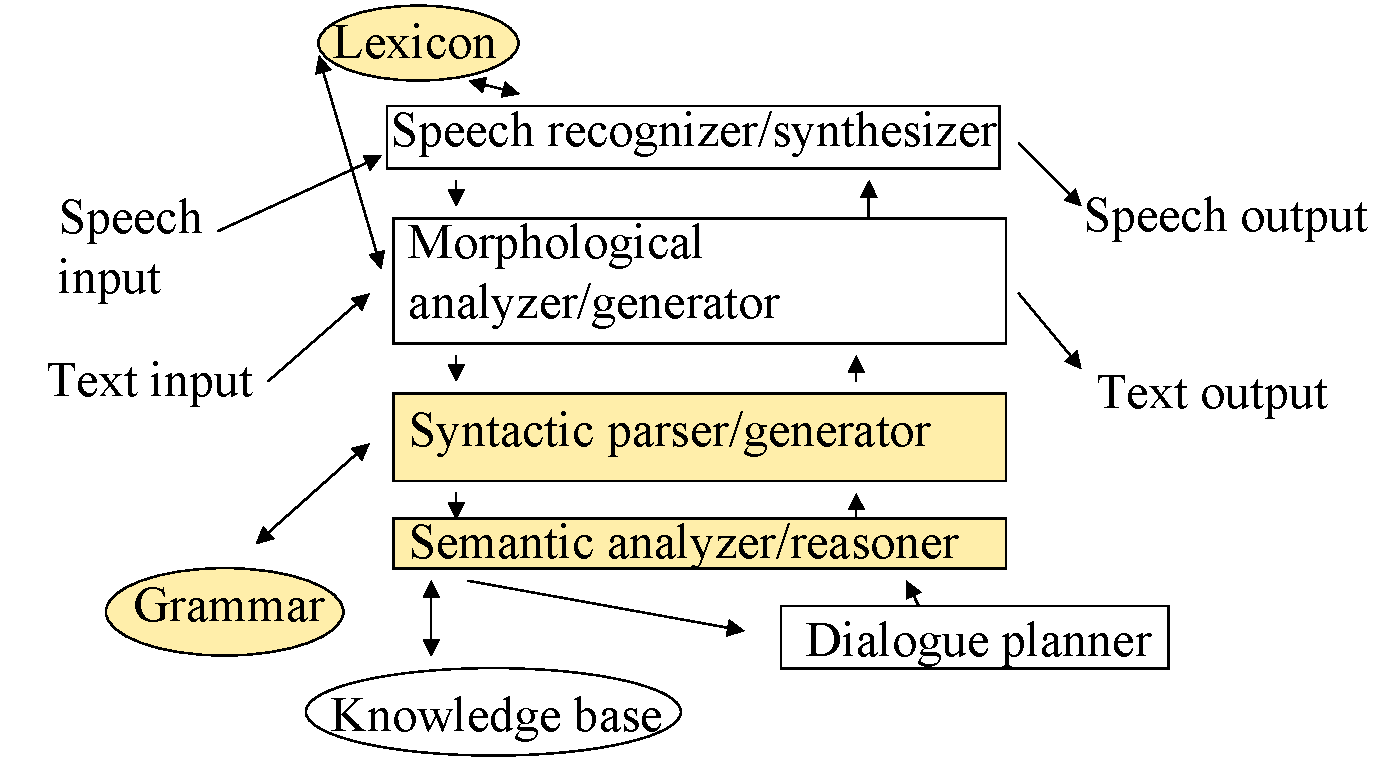
\includegraphics[width=\textwidth]{pics/syntax}

}





\frame{

\frametitle{Parts of speech}

\begin{itemize} 
 
\item \textit{dog} -- noun 
 
\item \textit{run} -- verb

\item \textit{the} -- determiner, definite article
 
\end{itemize} 
  

}





\frame{

\frametitle{Construction types}

\begin{itemize} 
 
\item \textit{the dog} -- noun phrase 
 
\item \textit{the dog ran} -- sentence

\item \textit{the thief [who saw the policeman] ran into the shop} --
  relative clause

\item \textit{I wonder [who saw the policeman]} -- embedded question
 
\end{itemize} 
  

}





\frame{

\frametitle{Grammars and grammar rules}

\begin{itemize} 
 
\item sentences may consist of a noun phrase followed by a verb phrase
  -- 
  \textit{S} $\rightarrow$ \textit{NP} \textit{VP} 
 
\item phrase structure grammars, context free grammars (\href{http://en.wikipedia.org/wiki/Chomsky_hierarchy}{Chomsky hierarchy})

\item are natural languages context free?

\item features \textit{*the dog run}, \textit{*the dogs runs}
 
\end{itemize} 
  

}





\frame{

\frametitle{Syntactic structures}

\begin{center}
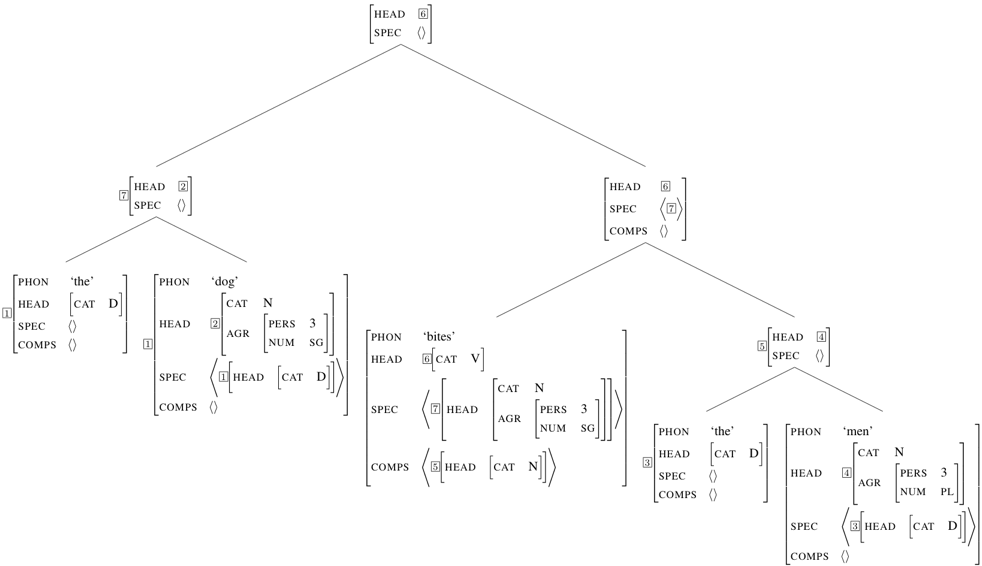
\includegraphics[scale=0.7]{pics/hpsg}

\footnotesize From \href{http://www.wellnowwhat.net/blog/?p=359}{here}.
\end{center}


}





\section{Semantics}


\frame{

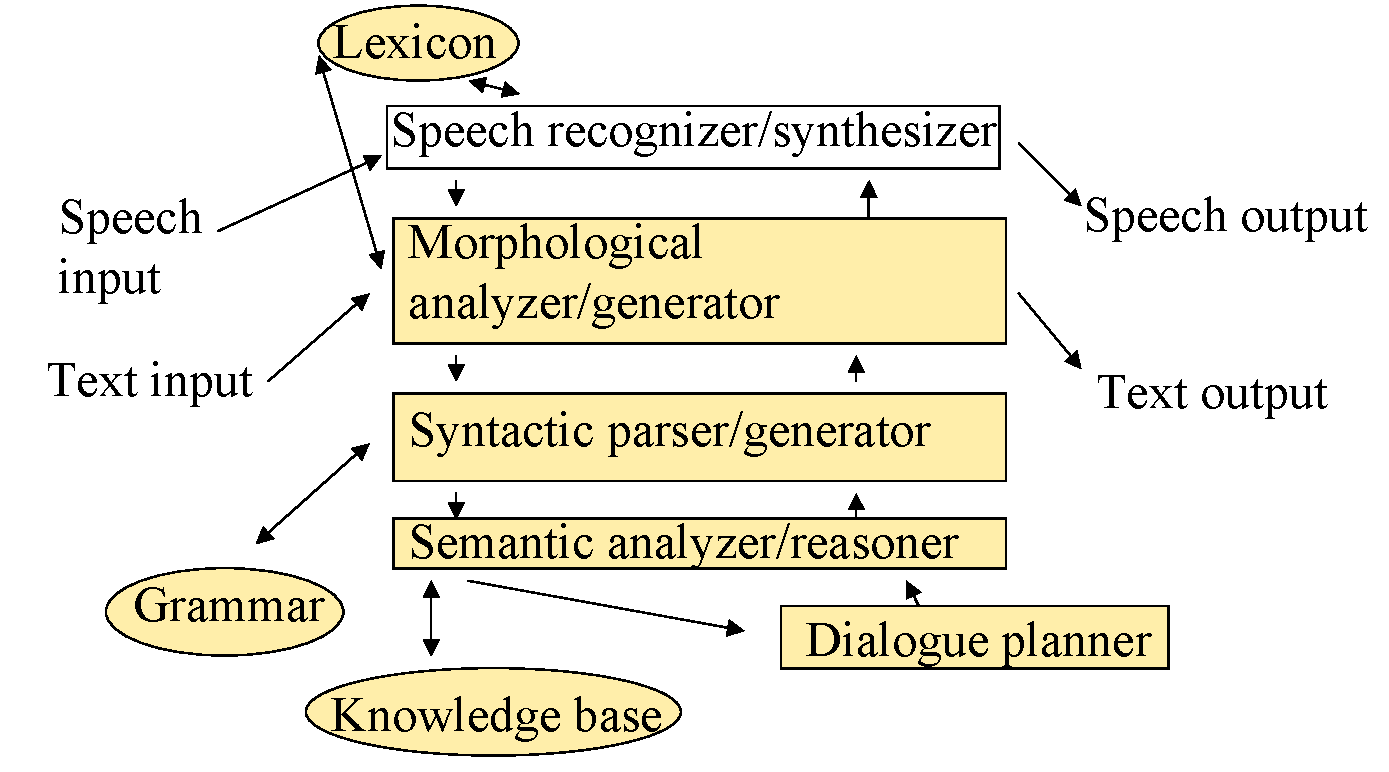
\includegraphics[width=\textwidth]{pics/semantics}

}

\frame{

\frametitle{Semantic properties and model theory}

\begin{itemize} 
 
\item ``to know the meaning of a (declarative) sentence is to know the
  conditions under which it would be true''
 
\item truth in a model 
 
\end{itemize} 
  

}





\frame{

\frametitle{Logic}

\begin{itemize} 
 
\item \href{http://en.wikipedia.org/wiki/Propositional\_logic}{propositional} logic 
 
\item \href{http://en.wikipedia.org/wiki/First\_order\_logic}{first order} logic

\item predicates, constants, variables, quantifiers \\
  \begin{itemize}
    \item Every television presenter has a secret. \\
      $\forall\,  x. (\mbox{\textsf{television\_presenter}}(x) \Rightarrow \exists\,  y. (\mbox{\textsf{secret}}(y) \wedge \mbox{\textsf{have}}(x,y)))$\\
      $\exists\,  y. (\mbox{\textsf{secret}}(y) \wedge \forall\,  x. (\mbox{\textsf{television\_presenter}}(x) \Rightarrow \mbox{\textsf{have}}(x,y)))$
    \end{itemize}

\item model theory for logic

\item inference
\end{itemize} 
  

}





\frame{

\frametitle{Pragmatics}

\begin{itemize} 
 
\item language in use 
 
\pause \item speech acts (assert, query, \ldots)

\pause \item language in context (deictic pronouns \textit{I}, \textit{you},
  but also demonstratives (\textit{this}, \textit{that}) and tense)

\pause \item presuppositions (\textit{my wife is coming} $\rightarrow$
   \textit{I have a wife}, \textit{my wife isn't coming} $\rightarrow$  \textit{I have a wife})
 
\end{itemize} 
  

}





\frame{

\frametitle{Dynamic meaning}

\begin{center}
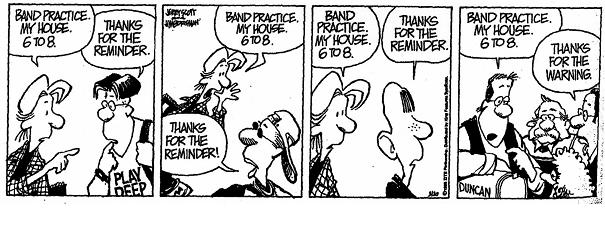
\includegraphics[scale=0.7]{pics/pragmatics}

From \href{http://zentrum.virtuos.uos.de/wikifarm/fields/english-language/field.php/Pragmatics/Pragmatics}{here}.
\end{center}


}





\section{Lexicon}

\frame{

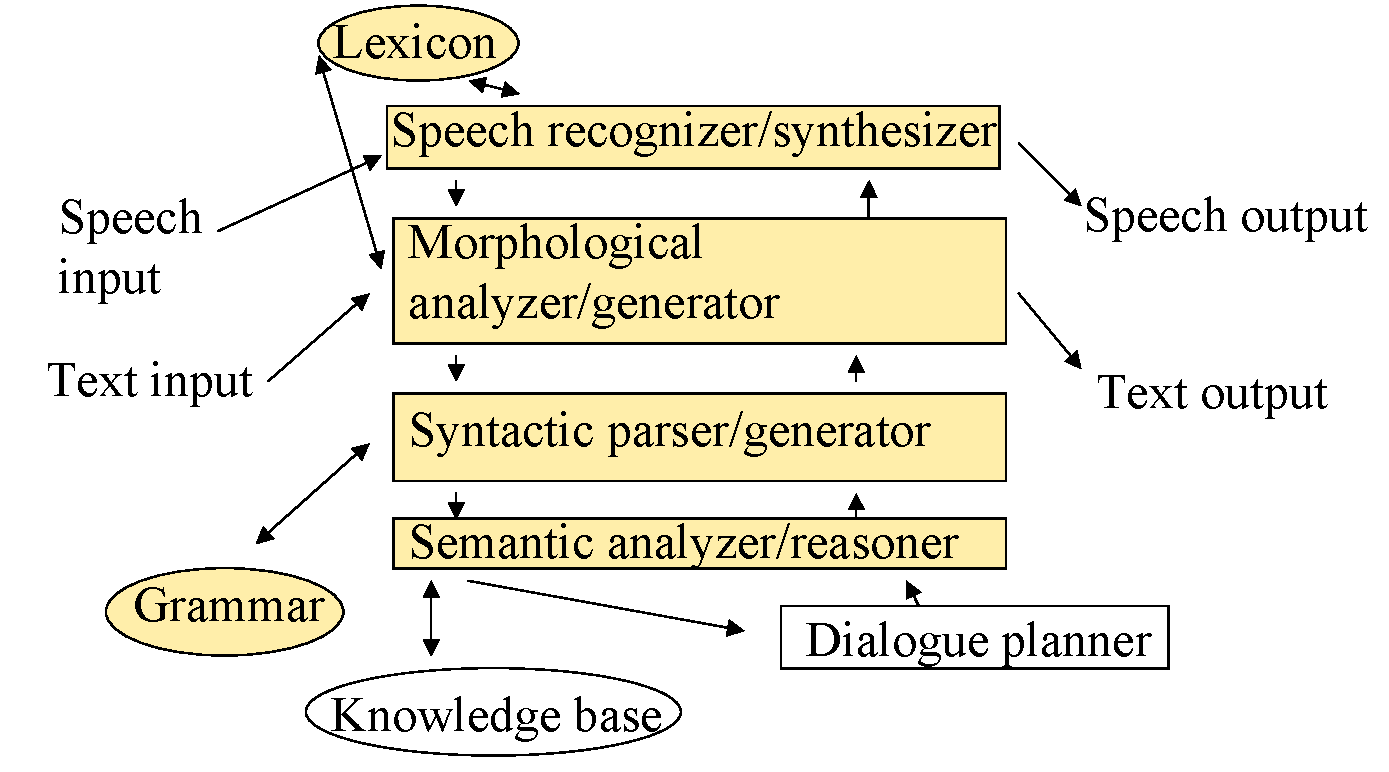
\includegraphics[width=\textwidth]{pics/lexicon}

}





\frame{

\frametitle{Words and phrases}

\begin{itemize} 
 
\item ``the lexicon is a list of words'' 
 
\pause \item seems also to include phrases -- \textit{look up (the number)},
  \textit{keep track of (the score)}, \textit{kick the bucket}

\pause \item more information than just the words: phonology, morphology,
  syntax semantics

 
\end{itemize} 
  

}





\section{A broader view}

\frame{

\frametitle{Some other areas of linguistics}

\ldots which may be relevant to language technology:

\bigskip

\begin{itemize} 
 
\item historical linguistics  
\item comparative linguistics and language typology 
\item dialect studies 
\item sociolinguistics 
\item psycholinguistics (language acquisition, human language processing)  
\end{itemize} 

} 





\frame{

\frametitle{Language variation and universals}

\begin{itemize} 
 
\item languages are different but there's a limit on how different
  they are  
\item language universals

\begin{itemize}  
\pause \item Sam read the books in the living-room 
 
\pause \item Did Sam read the books in the living-room?

\pause \item *Living-room the in books the read Sam?

\pause \item Sam read the books which are in the living-room

\pause \item Which room did Sam read the books in \_\_\_\_?

\pause \item *Which room did Sam read the books which are in \_\_\_\_?
 
\end{itemize} 
   
 
\end{itemize} 
  
} 





\frame{

\frametitle{Everybody can talk}

\begin{itemize}  
\pause \item \ldots except perhaps because of sickness, developmental
  characteristics or unusual social conditions
 
\pause \item native speakers

\pause \item linguistic (un)consciousness (lexicon vs grammar rules)
 
\end{itemize} 

}





\frame{

\frametitle{Language acquisition}

\begin{center}
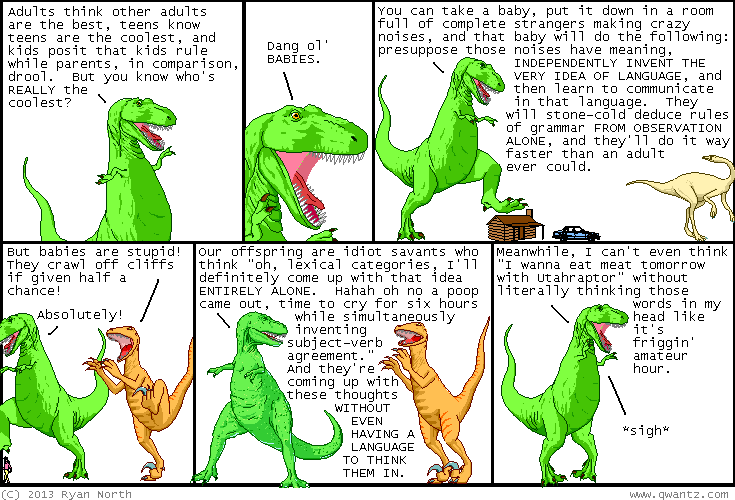
\includegraphics[scale=0.66]{pics/language-acquisition}

From \href{http://www.qwantz.com/index.php?comic=2479}{here}.
\end{center}


}





\frame{

\frametitle{Linguistics and psychology}

\begin{itemize} 
 
\item developmental psychology 
 
\item human processing

\pause \item should language technologists be concerned with this?

\pause \item should language technology systems imitate humans?




\end{itemize} 

}





\frame{

\frametitle{Why is linguistics (and language technology) difficult?}

\begin{itemize} 
 
\item natural languages are complex  
\pause \item interaction with context

\pause \item multimodality, body language 
\pause \item difficult to give a precise scientific theory of our linguistic behaviour  
\end{itemize} 

}





\frame{

\frametitle{Human languages and other languages}

\begin{itemize} 
 
\item animal languages  
\item artificial languages (logic, programming languages)

\item human languages
 
\end{itemize} 
}





\frame{

\frametitle{Some properties of human languages}

\begin{itemize} 
 
\pause \item displacement (talking about things not present, time/tense,
  negation, (im)possibilities)  
\pause \item arbitrary (compare different words for common objects in
  unrelated languages) 
\pause \item productive (take any sentence, can you create a longer
sentence which contains it?) 
\pause \item discrete (digitisation)  
\end{itemize} 

}        



\end{document}
